\documentclass[12pt]{article}
\usepackage[utf8]{inputenc}
\usepackage[T2A]{fontenc}
\usepackage[mongolian]{babel}
\usepackage{graphicx}
\graphicspath{{image/}}
\title{Сургуулийн хуудас}
\author{О.Болортуяа B140920086}

\begin{document}
	\maketitle
		\section{Системийн шаардлага}
		\begin{itemize}
			\item Систем нь бүрэн гүйцэт зохион байгуулагдсан байх ёстой
			\item Системийг ашиглахын тулд заавал сүлжээнд холбогдсон байх.
			\item Хэрэглэгч нэвтрэхэд оилгомжтой байх
			\item Гаргасан хийх  жагсаалтуудыг бусдад ойлгомжтой харуулах
		 	
		\end{itemize}
	\section{Системийн хэрэглэгчид}
	\begin{itemize}
		\item Бүх хэрэглэгчид
	\end{itemize}
\section{Функционал шаардлага}
\begin{enumerate}
	\item menu
		\item Сургуулийн хичээлийн жагсаалт
	\item  pro зураг солих
		\item cover солих
		\item Нийтлэл
		\item Бүлгэм
	\item event, арга хэмжээ
		\item үнэлгээ өгөх
		\item шүүмж
		\item шинэ хуудасруу зочлох
		\item тухай
	\end{enumerate}
\section{Функциональ бус шаардлага}	
\begin{itemize}
	\item Хуудас хооронд хурдан шилжих
	\item Хүн удаан харахад нүд ядрахгүй байх
	\item шинэ шинэ мэдээлэлтэй байх 
	\item Системийн загвар хүнд ойлгомжтой байх\part{title}
\end{itemize}
\section{use case diagram}
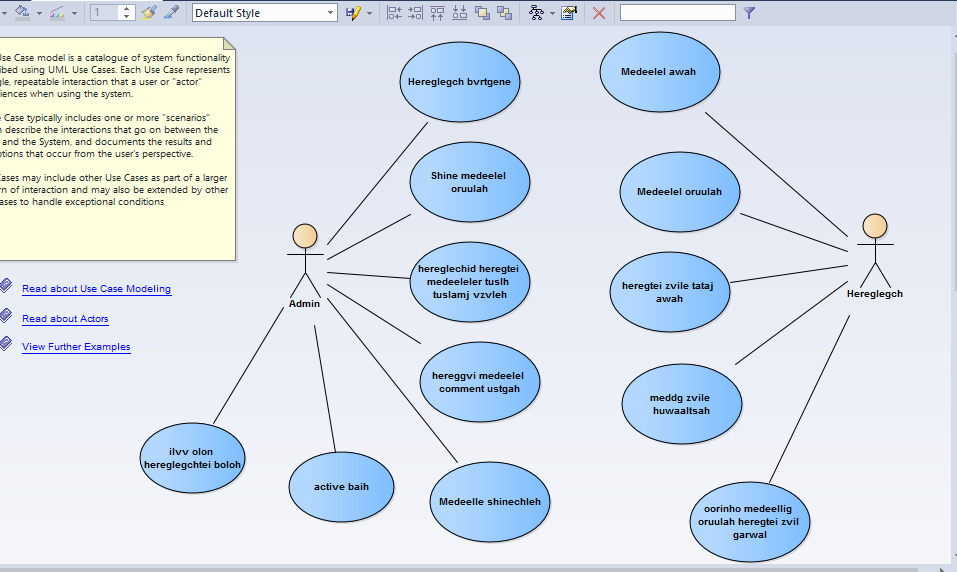
\includegraphics[width=\textwidth]{Usecase}

\end{document}